\chapter{Paper} \label{c:Paper}
In this chapter we will examine the topic of the paper \textit{Stable Neo-Hookean Flesh Simulation}. The goal of the paper was to model deformations for virtual characters that have human-like features.

\section{Deformation}
Graphically we can imagine a deformation with the help of a deformation map. In Fig. \ref{fig:deformationmap} we have on the left side an ellipse that signifies an object in its rest state. On the right side in the same image we can see the ellipse in a deformed state. We can map each point from its rest state to the deformed one with the help of the function $\phi$.

\begin{figure}[!htbp]
	\centering
	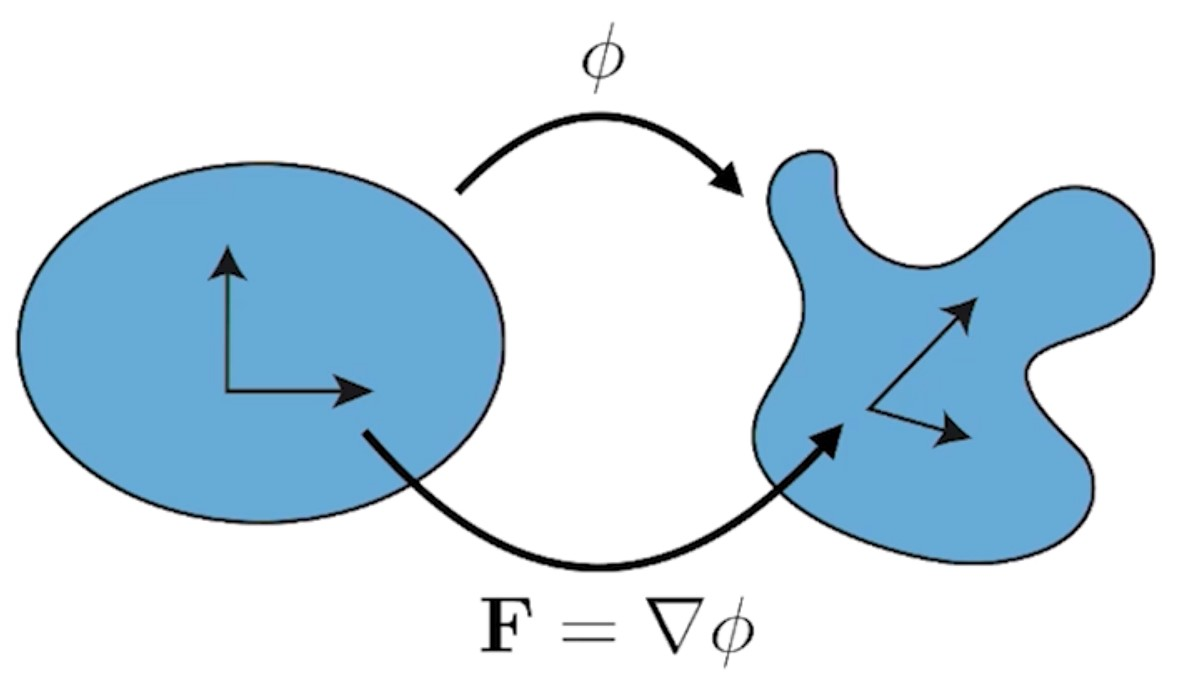
\includegraphics[width=0.5\textwidth]{resources/deformation_map}
	\caption{Deformation Map {\cite{STREAM2018}}}
	\label{fig:deformationmap}
\end{figure}

When applying a force over an object naturally the object itself undergoes a deformation. In the following we will be consistent with most previous literature in continuum mechanics and use the term strain as a measure of deformation and stress as the force per unit area.

\begin{addmargin}[2cm]{2cm}
\textit{Strain = measure of deformation}  \\
\textit{Stress = force per unit area} 
\end{addmargin}


\section{Deformation Gradient}

The deformation gradient $F$ is also shown in Fig. \ref{fig:deformationmap}. It offers us a measurement of the deformation. With its help we can amongst other things calculate the volume and length change an object undergoes during a deformation.
For our needs we define the deformation gradient as followed:

\[ F =  \begin{bmatrix}
  		f_0 & f_3 & f_6 \\
  		f_1 & f_4 & f_7 \\
  		f_2 & f_5 & f_8 \\
		\end{bmatrix} 
\]


Measure for the deformation, length and volume change etc.
Nonlinear deformations
http://www.continuummechanics.org/deformationgradient.html
also add some examples

\section{Material Constants}

Naturally the properties of the material the object consists of play an important rule in the deformation process. The two constants $\mu$ and $\lambda$ that are crucial for us are called \textit{Lamé Parameters}. The formula in which they appear is called \textit{Poisso's Ratio} and is of the following form:

\[ \sigma =  \frac{\lambda}{2(\lambda + \mu)} \in [-1, 0.5] \]

The poisson's ratio is of importance for us since it characterizes the materials resistance to volume change. Usually the poisson's ratio of a material is positive.
\\
For the simulation of human-like flesh we have to choose a poisson's ratio that is almost 0.5 to get realistic results.
\\ further reading: http://silver.neep.wisc.edu/~lakes/PoissonIntro.html


\section{Deformation Energy}

In order to get a convincing simulation of high quality we must choose an appropriate energy. In the case of modelling deformations on human-like characters we have to choose an elastic energy. The key property that makes an energy elastic is that if all the forces that are applied over an object add up to zero the object must come back to its rest shape.
\\
The energy then has to be minimized to get the results we want.

\begin{definition}
  This is a definition.
\end{definition}



